% ACCV 2026 Workshop on Trustworthy Foundation Models in Medical Imaging (TrustFMI).
% Draft scaffold on the Springer llncs class; move into the official ACCV 2026
% template before submission and keep splncs04. Double-blind: no names, no links.
\documentclass[runningheads]{llncs}
\usepackage{graphicx}
\usepackage{booktabs}
\usepackage{amsmath,amssymb}
\usepackage{multirow}
\usepackage{xcolor}
\usepackage[hidelinks]{hyperref}
% Numbers that update when the last jobs finish are wrapped in \pending{}.
\newcommand{\pending}[1]{\textcolor{blue}{#1}}
\newcommand{\todo}[1]{\textcolor{red}{[TODO: #1]}}

\begin{document}

\title{Protect the Decoder: Representation-Preserving Adaptation and Failure Detection for Far-OOD MedSAM}
\titlerunning{Protect the Decoder}
\author{Anonymous Submission}
\authorrunning{Anonymous}
\institute{Paper ID \todo{OpenReview ID}}

\maketitle

\begin{abstract}
Parameter-efficient adaptation of MedSAM to one imaging domain can leave it worse than zero-shot on distant domains, a collapse that earlier work linked to drift of the mask decoder's representations from the base model. We intervene on that mechanism: a centred kernel alignment (CKA) loss pulls the adapted decoder's activations on a 32-image out-of-distribution probe back toward the base decoder during LoRA training on dermoscopy. Over three seeds the regulariser raises tight-box Dice by 0.05 on breast ultrasound and 0.10 on mammography with no in-domain cost; the same anchor on the image encoder alone lowers far-OOD Dice, and anchoring encoder and decoder together gives the largest gain. Varying the adaptation budget from 50 to 2595 images shows that LoRA falls below zero-shot far-OOD already at 250 images, whereas decoder-only and encoder-only adaptation never do. Finally, the per-image drift of the decoder's upscaled mask embedding detects far-OOD failures of parameter-efficient adapters with AUROC 0.95 on ultrasound and 0.82 on mammography, where the decoder's own IoU estimate is at chance, while the IoU estimate is informative for full fine-tuning. Far-OOD robustness of adapted MedSAM is decided at the decoder, and it can be both protected and monitored there.
\keywords{Medical image segmentation \and Foundation models \and Parameter-efficient fine-tuning \and Out-of-distribution robustness \and Failure detection}
\end{abstract}

\section{Introduction}
\label{sec:intro}

MedSAM~\cite{ma2024medsam} adapts the Segment Anything Model~\cite{kirillov2023sam} to medical images and is routinely fine-tuned again for a target modality. Parameter-efficient methods such as LoRA~\cite{hu2022lora} and visual prompt tuning~\cite{jia2022vpt} make this cheap, but a prior comparison on a four-dataset drift ladder showed that the cheapest methods are also the most fragile: LoRA trained on dermoscopy gains in-domain accuracy and then loses 0.18 Dice relative to zero-shot MedSAM on mammography, while decoder-only and full fine-tuning keep their far-OOD accuracy~\cite{prior2026safer}. The same study found that the loss correlates with how far the mask decoder's representations move from the base model, measured by centred kernel alignment (CKA)~\cite{kornblith2019cka}, and that encoder-side movement does not predict it. That was a correlation over checkpoints; this paper asks whether it is a mechanism that can be acted on. First, does regularising the decoder toward the base model during adaptation reduce far-OOD collapse, and is the decoder specifically the locus? We add a CKA loss on a 32-image out-of-distribution probe and compare hooks on the decoder, on the encoder, and on both. Second, does the collapse scale with the adaptation budget? We train three adapters on nested subsets of 50, 250 and 1000 images at a fixed step budget. Third, can an adapted model flag its own far-OOD failures at inference? We compare two label-free per-image signals: the IoU estimate SAM's decoder already produces, and the drift of the decoder's upscaled mask embedding relative to the base model on the same image and prompt.

Our contributions are:
\begin{enumerate}
  \item a CKA-regularised LoRA with an OOD-only probe, evaluated over three seeds and five prompt-jitter levels, and a hook-placement ablation showing that encoder-only anchoring hurts, decoder anchoring helps, and anchoring both is best;
  \item an adaptation-budget study showing that LoRA's far-OOD loss appears at 250 training images and does not recover with more data, while decoder-only and encoder-only adaptation stay above zero-shot at every budget;
  \item a per-image failure detector based on decoder drift that reaches AUROC 0.95 and 0.82 on the two far-OOD sets for LoRA, together with the finding that the decoder's IoU head is uninformative for parameter-efficient adapters but informative for full fine-tuning.
\end{enumerate}

\section{Related Work}
\label{sec:related}

\paragraph{Adapting SAM to medical images.}
MedSAM fine-tunes SAM's encoder and decoder on over a million image-mask pairs with box prompts~\cite{ma2024medsam}; SAM-Med2D adds encoder adapters and retrains the decoder interactively~\cite{cheng2023sammed2d}. Downstream users adapt these models again to one modality with LoRA~\cite{hu2022lora}, prompt tokens~\cite{jia2022vpt}, or by unfreezing the decoder. The prior study we build on compared seven such strategies on a dermoscopy to ultrasound to mammography ladder and found that LoRA and prompt tuning collapse at the far end while decoder-only and full fine-tuning do not~\cite{prior2026safer}. We take its testbed and diagnosis as given and study interventions.

\paragraph{Feature distortion under fine-tuning.}
Fine-tuning a good pretrained extractor can distort its features and underperform linear probing out of distribution, and in a linear model the distortion persists along the whole fine-tuning trajectory~\cite{kumar2022finetuning}; the same mechanism has been analysed for LoRA through the neural tangent kernel~\cite{tomihari2024ntk}. The remedies form one family: choose which layers to tune by the type of shift~\cite{lee2023surgical}, interpolate fine-tuned and zero-shot weights~\cite{wortsman2022wiseft}, or penalise the change of pretrained features directly, with a feature-protection loss for CLIP~\cite{tan2024protection} or a penultimate-layer distance that preserves OOD detection after fine-tuning~\cite{zhang2025oodreg}; for MedSAM, adapting image embeddings at test time avoids parameter updates altogether~\cite{chen2025tta}. Preserving pretrained representations is therefore not new. Those results concern a single extractor read out by a linear head, and the quantity they preserve is the total change of its features. A promptable segmenter has a second network between encoder and output, and our question is not whether representations move but where: our results place the loss and recovery of robustness in the decoder and show that encoder movement by itself is benign. We use linear CKA~\cite{kornblith2019cka} as a differentiable anchor to the model's own initialisation on a fixed probe batch.

\paragraph{Failure detection for segmentation.}
Estimating segmentation quality without ground truth ranges from reverse classification accuracy~\cite{valindria2017rca} to recent benchmarks of confidence-based failure detectors for medical segmentation~\cite{zenk2024failure}. SAM's decoder emits a scalar IoU estimate for each mask~\cite{kirillov2023sam}, but its behaviour after adaptation has not been examined. We evaluate it against a detector derived from the mechanism studied here.

\section{Method}
\label{sec:method}

$f_\theta$ denotes MedSAM with image encoder $E_\theta$ and mask decoder $D_\theta$, $\theta_0$ its released weights and $\theta$ the weights during adaptation; prompts are single boxes.

\subsection{CKA-regularised adaptation}
\label{sec:cka_loss}

For activation matrices $X \in \mathbb{R}^{n \times p}$ and $Y \in \mathbb{R}^{n \times q}$ with centred columns, linear CKA is
\begin{equation}
  \mathrm{CKA}(X, Y) = \frac{\lVert Y^\top X \rVert_F^2}{\lVert X^\top X \rVert_F \,\lVert Y^\top Y \rVert_F} \in [0,1],
\end{equation}
invariant to orthogonal transformation and isotropic scaling of either side~\cite{kornblith2019cka}. Let $P$ be a fixed probe batch of $n$ images with boxes and $A_\ell(\theta; P)$ the activation captured by a forward hook at layer $\ell$, one row per probe image. With $A_\ell(\theta_0; P)$ cached once, the training objective is
\begin{equation}
  \mathcal{L} = \mathcal{L}_{\text{task}} + \lambda \sum_{\ell \in H} w_\ell \bigl(1 - \mathrm{CKA}\bigl(A_\ell(\theta_0; P), A_\ell(\theta; P)\bigr)\bigr),
  \label{eq:loss}
\end{equation}
where $H$ is the set of hooked layers, $w_\ell$ per-layer weights and $\mathcal{L}_{\text{task}}$ the equally weighted sum of binary cross-entropy and soft Dice. The probe forward runs every fourth step with $\lambda$ multiplied by four, which keeps the expected regularisation gradient per step and quarters its cost; CKA terms are computed in single precision. The probe is OOD-only: 16 breast-ultrasound and 16 mammography images drawn once from the training splits of those datasets and absent from every evaluation set, each with a synthetic centred box covering half the image. No in-domain images are included, because the task loss already governs in-domain behaviour and an in-domain anchor competes with it. We use $\lambda = 10$ (preliminary sweep over $\{0.1, 1, 10\}$).

\subsection{Hook placement}
\label{sec:hooks}

\emph{Decoder} hooks capture the output of the decoder's upscaling block ($32 \times 256 \times 256$), the IoU prediction head and the mask logits, with $w_\ell = 0.8$, $1.5$ and $1.0$, following the strength of the per-layer correlation reported in prior work~\cite{prior2026safer}. \emph{Encoder} hooks capture the neck output ($256 \times 64 \times 64$) and the outputs of the last two transformer blocks ($64 \times 64 \times 768$), each with $w_\ell = 1$. \emph{Both} is the union. Every configuration backpropagates through the encoder, where the LoRA weights live; the positions differ only in which representation is anchored.

\subsection{Adaptation-budget protocol}
\label{sec:budget}

One fixed permutation of the training set (seed 0) supplies its first 50, 250 and 1000 images, so smaller budgets are prefixes of larger ones and every method sees identical images. Each run performs 6000 optimiser steps at batch size one under a cosine schedule, validating every 500 steps and keeping the best checkpoint; the full-data point is each method's seed-0 checkpoint. Prompts are tight.

\subsection{Per-image failure signals}
\label{sec:detector}

For a test image $x$ with box $b$, two label-free signals are available. The first is the decoder's IoU estimate $\hat{u}(x, b)$, a scalar SAM predicts alongside each mask~\cite{kirillov2023sam} and that adaptation updates with the rest of the decoder. The second is the decoder drift
\begin{equation}
  d(x, b) = 1 - \mathrm{CKA}\bigl(U_{\theta_0}(x, b),\, U_{\theta}(x, b)\bigr),
  \label{eq:drift}
\end{equation}
where $U(x,b) \in \mathbb{R}^{65536 \times 32}$ is the decoder's upscaled mask embedding for that image and prompt, with the $256 \times 256$ positions as samples and the 32 channels as features. The same quantity on the encoder's neck output ($4096 \times 256$) gives an encoder drift. Computing them costs one extra base decoder forward per image, plus a base encoder forward when the encoder was adapted. A failure is a prediction with Dice below 0.5 (0.3 to 0.7 in a sensitivity check); both signals are scored by AUROC and AUPRC (high drift or low $\hat{u}$ positive) and by the recall and residual failure rate obtained when the top fraction of images by signal is flagged for review, and $\hat{u}$ is compared with the true IoU by a ten-bin expected calibration error.

\section{Experimental Setup}
\label{sec:setup}

\paragraph{Drift ladder.}
All adaptation uses the ISIC 2018 dermoscopy training set~\cite{codella2019isic} (2594 training, 100 validation, 1000 test images). Evaluation adds PH2~\cite{mendonca2013ph2} (200 dermoscopy images from another clinic, near-OOD), BUSI~\cite{aldhabyani2020busi} (647 benign and malignant breast-ultrasound images, far-OOD) the 362 CBIS-DDSM test mammograms~\cite{lee2017cbis} with mass and calcification masks merged per image (far-OOD), and, as a held-out check used once, the 269 annotated mammograms of DMID~\cite{oza2024dmid} with their lesion masks (far-OOD, a second mammography source). Images are resized to $1024 \times 1024$; box prompts come from the ground-truth mask, tight at evaluation unless stated.

\paragraph{Methods.}
The seven strategies are those of the prior study~\cite{prior2026safer}: zero-shot MedSAM; decoder-only fine-tuning; VPT-shallow and VPT-deep (ten prompt vectors at the encoder input or at every block, decoder trainable); LoRA with rank 8 on the fused query-key-value projection of all twelve encoder blocks, decoder trainable; encoder-only LoRA with rank 28 on every encoder linear layer, decoder frozen; and full fine-tuning. All use AdamW with a cosine schedule and mixed precision, with learning rates $5 \times 10^{-4}$ (LoRA, prompts), $10^{-4}$ (decoder-only) and $10^{-5}$ (full). Regularised runs are LoRA plus Eq.~\eqref{eq:loss}. Training regime pm20 jitters each box corner uniformly within $\pm 20$ pixels, pm0 uses tight boxes, and rand100 draws the jitter magnitude uniformly from $[0, 100]$ per step. A run takes six epochs on one 48\,GB GPU.

\paragraph{Evaluation.}
We report Dice, IoU and HD95 (pixels on the 1024 grid). Prompt robustness expands each side of the tight box outward by an amount drawn uniformly from $[0, p]$ pixels, $p \in \{20, 50, 100, 200\}$, with one draw per image seeded on its identifier so all models see identical boxes. Multi-seed comparisons use seeds 0 to 2 and a paired Wilcoxon signed-rank test over per-image Dice, pairs matched on seed and image, Holm-corrected over the four datasets.

\paragraph{Prior results.}
The prior study reported tight-box zero-shot Dice of 0.823 and 0.692 on BUSI and CBIS-DDSM, LoRA below zero-shot at 0.780 and 0.509 against decoder-only and full fine-tuning at 0.894 to 0.901 and 0.828, and decoder-side CKA correlating with far-OOD Dice at $\rho = 0.76$ against $\rho = 0.09$ for the encoder~\cite{prior2026safer}; these baselines are not re-derived here.

\section{Results: CKA Regularisation}
\label{sec:res_cka}

\begin{table}[tbp]
  \centering
  \caption{LoRA with and without the decoder CKA loss, both trained with 20\,px jitter, tight-box evaluation, mean $\pm$ std over three seeds; $\Delta$HD95 in pixels. $p$: paired Wilcoxon over per-image Dice at 20\,px evaluation jitter, pairs matched on seed and image, Holm-corrected.}
  \label{tab:cka}
  \begin{tabular}{lcccrr}
\toprule
Dataset & no-CKA Dice & CKA Dice & $\Delta$Dice & $\Delta$HD95 (px) & $p$ (Holm) \\
\midrule
ISIC (ID) & 0.949 $\pm$ 0.002 & 0.952 $\pm$ 0.002 & +0.003 & -0.3 & $<$0.001 \\
PH2 (near-OOD) & 0.951 $\pm$ 0.001 & 0.954 $\pm$ 0.002 & +0.003 & -0.4 & $<$0.001 \\
BUSI (far-OOD) & 0.774 $\pm$ 0.032 & 0.826 $\pm$ 0.008 & +0.051 & -96.1 & $<$0.001 \\
CBIS-DDSM (far-OOD) & 0.437 $\pm$ 0.095 & 0.541 $\pm$ 0.095 & +0.104 & -152.4 & $<$0.001 \\
\bottomrule
\end{tabular}

\end{table}

\paragraph{Multi-seed effect.}
Table~\ref{tab:cka} gives the main comparison. The decoder CKA loss leaves in-domain and near-OOD Dice within 0.003 and raises far-OOD Dice by 0.051 on BUSI and 0.104 on CBIS-DDSM, with HD95 falling by 96 and 152 pixels: the regulariser removes the boundary failures of unregularised LoRA rather than small overlap losses. The BUSI gain is stable across seeds (std 0.008 against 0.032 without the loss); on CBIS-DDSM the seed spread is large for both models (std 0.095) but the gain holds in every seed, and the paired test is significant on all four datasets with a median per-image gain of 0.088 on CBIS-DDSM. With tight-box training the loss gives smaller same-signed gains (0.033, 0.027; seed 0); with rand100 training it hurts (0.059 and 0.032 lower), so the two regularisers compound at mild jitter and conflict under heavy jitter.

\begin{figure}[tbp]
  \centering
  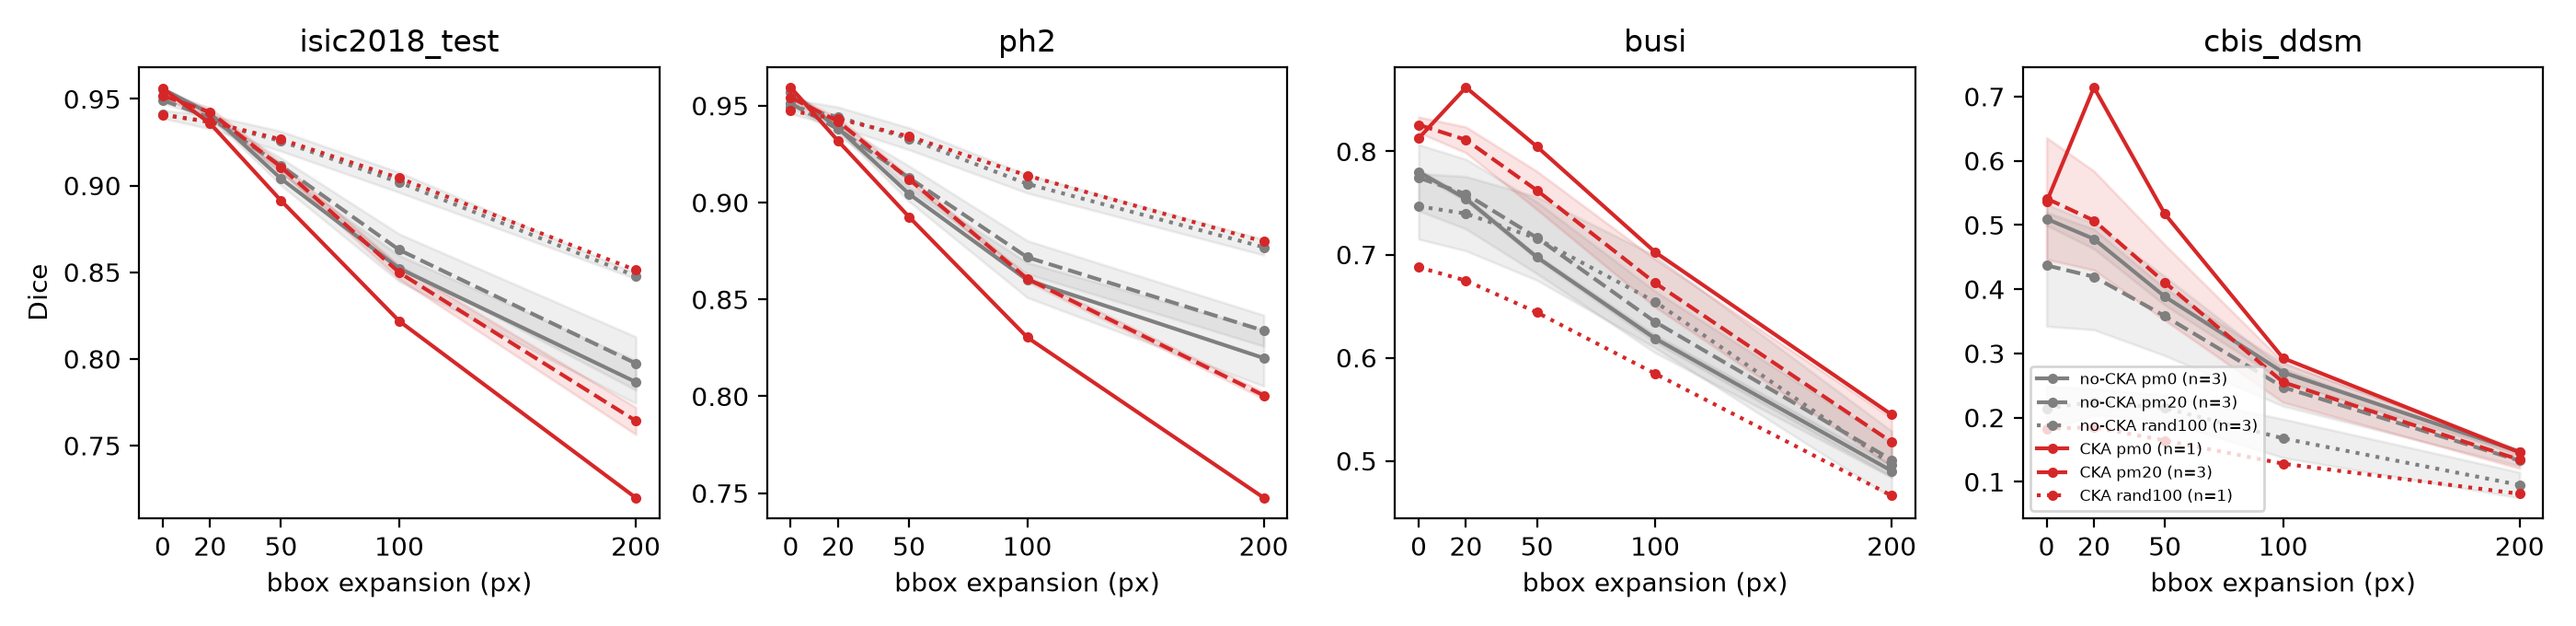
\includegraphics[width=0.86\linewidth]{figures/robustness_six_curves.png}
  \caption{Dice against outward box expansion for LoRA with (red) and without (grey) the decoder CKA loss under three training regimes: tight (solid), 20\,px jitter (dashed), random jitter up to 100\,px (dotted). Bands: one std over three seeds where available.}
  \label{fig:curves}
\end{figure}

\paragraph{Prompt robustness.}
In Fig.~\ref{fig:curves} the regularised pm20 model is the best of the six on both far-OOD sets at every expansion, with an advantage that narrows as boxes loosen: the paired gain on BUSI is 0.053, 0.046, 0.038 and 0.017 at 20, 50, 100 and 200\,px, and on CBIS-DDSM 0.088, 0.052, 0.008 and not significant. On the dermoscopy sets the sign flips beyond 50\,px (0.013 lower at 100\,px, 0.033 at 200\,px, $p < 10^{-20}$): anchoring to a base trained with tight boxes inherits its sensitivity to loose boxes in-domain. The rand100 regime is the other side of the trade, buying in-domain prompt robustness at a far-OOD price that the CKA loss makes worse.

\begin{figure}[tbp]
  \centering
  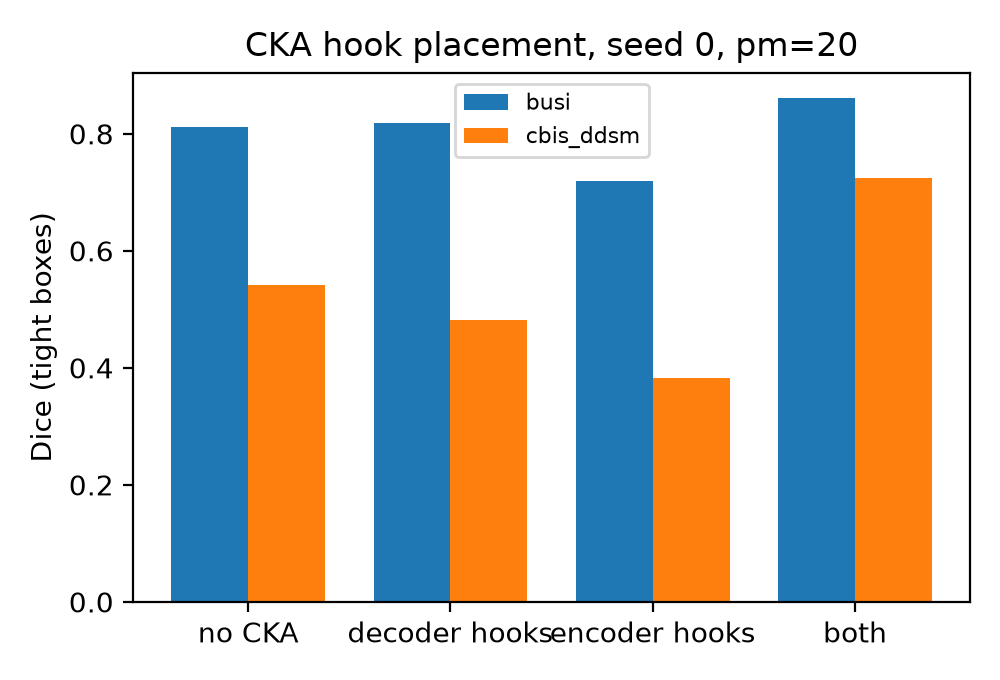
\includegraphics[width=0.36\linewidth]{figures/hook_ablation.png}
  \caption{Hook placement (LoRA, 20\,px training, tight-box evaluation): far-OOD Dice with no regulariser, decoder hooks, encoder hooks, and both; bars are means over seeds 0 to 2 with one std, dots the individual seeds.}
  \label{fig:hooks}
\end{figure}

\paragraph{Where the anchor must be.}
Figure~\ref{fig:hooks} separates the two halves of the model over three seeds. With the loss on encoder activations alone, far-OOD Dice falls below the unregularised baseline in every seed, to $0.725 \pm 0.023$ on BUSI and $0.357 \pm 0.059$ on CBIS-DDSM (paired per-image loss 0.037 and 0.055, $p < 10^{-4}$), at unchanged in-domain Dice. Decoder hooks give the gains of Table~\ref{tab:cka}. Anchoring both is best: $0.834 \pm 0.027$ and $0.626 \pm 0.098$, a paired gain over decoder hooks of 0.010 and 0.088 (median 0.062, $p < 10^{-4}$) and over no regulariser of 0.062 and 0.175, with 76 percent of CBIS-DDSM images improved, for a 0.003 in-domain cost. The seed spread on CBIS-DDSM is large for every arm (the best single run, seed 0 with both hooks, reaches 0.725; two independent trainings of the tight-box decoder-hook configuration reached 0.536 and 0.779), so we report paired statistics rather than best seeds. The decoder is the locus, and the encoder anchor helps only once the decoder is anchored too.

\paragraph{A second mammography source.}
On DMID, which no model or probe has seen (269 images, tight boxes, table in the supplement), LoRA falls from a zero-shot 0.637 to 0.402 and VPT to 0.53 and 0.57, while decoder-only, encoder-only LoRA and full fine-tuning reach 0.727 to 0.733; the decoder anchor lifts LoRA to 0.697 (tight-box training) and 0.651 (both hooks), encoder hooks alone give 0.366. Every comparison matches CBIS-DDSM.

\section{Results: Adaptation Budget and Drift}
\label{sec:res_budget}

\begin{figure}[t]
  \centering
  
\includegraphics[width=0.94\linewidth]{figures/budget_curves.png}
  \caption{Adapters trained for a fixed 6000 steps on nested subsets (log axis), zero-shot dashed. Left: in-domain Dice. Centre: far-OOD Dice, mean of BUSI and CBIS-DDSM. Right: far-OOD representation drift ($1 - \mathrm{CKA}$ to the base model) of the decoder's upscaled embedding (circles) and of the encoder neck output (squares, dashed); decoder-only fine-tuning leaves the encoder untouched. Dice: mean and one std over three seeds at 50, 250 and 1000 images; the 2595-image point and the drift panel are seed 0.}
  \label{fig:budget}
\end{figure}

Figure~\ref{fig:budget} shows how the collapse depends on the budget and what moves inside the model when it happens. Decoder-only fine-tuning and encoder-only LoRA improve on both axes with every increase in budget and stay above the zero-shot far-OOD reference of 0.758 in every seed (0.840 to 0.861 and 0.811 to 0.864). LoRA with a trainable decoder is the only method that crosses it: already 0.02 to 0.05 below the others at 50 images ($0.790 \pm 0.027$, above zero-shot in each seed), it falls to $0.670 \pm 0.031$ at 250, below zero-shot in all three seeds, recovers to $0.774 \pm 0.019$ at 1000, above it in all three, and ends at 0.638 with all 2595 images, while its in-domain Dice rises monotonically. The drift panel says why. LoRA's far-OOD decoder drift triples between 50 and 250 images, from 0.12 to 0.36, exactly where its Dice collapses, and stays there. Decoder-only fine-tuning retrains every decoder weight yet keeps far-OOD decoder drift below 0.06 at all budgets; encoder-only LoRA moves the encoder twice as much as LoRA (encoder drift 0.25 against 0.12) and keeps far-OOD decoder drift below 0.09; in-domain decoder drift is similar for all three (0.07 to 0.15). The collapse is thus not a symptom of too little data (every budget receives 6000 steps), of decoder training as such, or of encoder movement as such: it appears when encoder and decoder adapt jointly without an anchor, as far-OOD decoder drift that more data does not undo. The dip at 250 images and the partial recovery at 1000 are reproduced in every seed; the recovery occurs at unchanged far-OOD decoder drift (0.35), so drift marks the onset of the collapse rather than tracking its depth.

\section{Results: Label-Free Failure Detection}
\label{sec:res_detect}

\begin{table}[tbp]
  \centering
  \caption{AUROC / AUPRC for detecting per-image failures (Dice below 0.5) at tight boxes: decoder drift (Eq.~\eqref{eq:drift}) versus the decoder's IoU estimate, on the two far-OOD sets and on DMID, which no model or probe has seen. Cells with fewer than 20 failures are omitted; drift is zero by construction for zero-shot. The 50\,px table is in the supplement.}
  \label{tab:detect}
  \begin{tabular}{lcccc}
\toprule
Method & \multicolumn{2}{c}{BUSI (far-OOD)} & \multicolumn{2}{c}{CBIS-DDSM (far-OOD)} \\
 & drift & IoU head & drift & IoU head \\
\midrule
Zero-shot & -- & -- & -- & 0.49 \\
Decoder-only FT & -- & -- & -- & -- \\
VPT-shallow & 0.93 & 0.69 & 0.70 & 0.49 \\
VPT-deep & 0.92 & 0.55 & 0.66 & 0.52 \\
LoRA & 0.95 & 0.72 & 0.82 & 0.46 \\
Encoder-only LoRA & -- & -- & -- & -- \\
Full FT & -- & -- & -- & -- \\
\bottomrule
\end{tabular}

\end{table}

\paragraph{Drift ranks LoRA's failures.}
LoRA's 61 failures among 647 BUSI images and 152 among 362 CBIS-DDSM images are detected with AUROC 0.95 and 0.82 (AUPRC 0.75 and 0.83), and its 175 failures among 269 DMID images with 0.76 (AUPRC 0.87). The result does not hinge on the failure threshold: for Dice thresholds from 0.3 to 0.7 the AUROC stays within 0.90 to 0.97 on BUSI and 0.73 to 0.82 on CBIS-DDSM, and under 50\,px jitter within 0.90 to 0.91 and 0.71 to 0.76 (supplement). Ranking quality translates into a review budget: flagging the 20 percent of BUSI images with the highest drift captures 87 percent of LoRA's failures and leaves a failure rate of 1.5 percent among the unflagged, from 9.4 percent overall; on CBIS-DDSM, where 42 percent of predictions fail, flagging half captures 79 percent and leaves 18 percent (risk-coverage table in the supplement). LoRA's IoU estimate is at or near chance on all three sets (0.72, 0.46, 0.60): after adaptation it collapses to a band between 0.4 and 0.6 regardless of mask quality.

\paragraph{VPT: on the ladder, not on DMID.}
VPT-shallow and VPT-deep failures are ranked by drift with AUROC 0.93 and 0.92 on BUSI and 0.70 and 0.66 on CBIS-DDSM, with the same threshold stability, but on DMID drift is at chance for both (0.47 and 0.45 over 93 and 110 failures) although its per-image spread there is as wide as on CBIS-DDSM. Drift is thus not a universal signal for parameter-efficient adapters: it is associated with LoRA's failures on every far-OOD set we have, and with VPT's on two of three.

\paragraph{The IoU estimate reacts to the prompt, not to the modality.}
Full fine-tuning and encoder-only LoRA fail on only 2 to 14 ladder images at tight boxes, too few to score, and their 51 and 52 DMID failures are missed by both signals (drift 0.59 and 0.69, IoU estimate 0.28 and 0.24). Under 50\,px jitter their 220 to 236 CBIS-DDSM failures are detected by the IoU estimate with AUROC 0.75 to 0.79 (0.87 to 0.89 on BUSI) while drift is below chance (0.23 to 0.36); zero-shot MedSAM is likewise served by its IoU head under jitter (0.87, 0.71) but not on DMID (0.47). The IoU head flags a poor box, which every model can sense, rather than a modality it has never seen. Drift marks predictions on which the adapted decoder has left the representation region the base model would use; it is uninformative once the decoder is retrained wholesale and moves for every image, and for the CKA-regularised models, whose anchor keeps drift low on failures and successes alike (0.35 and 0.46 on DMID). Neither signal is a self-assessment: drift needs a base-model forward, and both were validated against ground truth offline.

\section{Limitations and Conclusion}
\label{sec:limits}

The ladder is asymmetric: all models are adapted on dermoscopy, and we have not shown that the anchors help when a far-OOD set is the training domain. The budget study is single-seed, the hook ablation rests on \pending{one seed for the encoder and combined arms until the remaining runs complete}, the CKA loss adds about 30 percent to training time, and the drift detector doubles inference cost when the encoder is adapted. The regularised model also inherits the base's sensitivity to loose boxes in-domain.

Within those bounds the evidence points one way. Far-OOD failure of adapted MedSAM arises where the mask decoder's representations leave the base model's; an anchor there removes much of the failure at no in-domain cost, an anchor on the encoder alone makes it worse, and the size of that departure on a single image predicts whether the prediction has failed. Protecting the decoder during adaptation and monitoring it at inference are two uses of one cheap quantity.

% % Camera-ready only. Do not include in the anonymous submission.
\section*{Declarations}
\paragraph{Data availability.} All four datasets are public (ISIC 2018, PH2, BUSI, CBIS-DDSM). Configuration files, training and evaluation code, per-image result files and figure scripts are released at \todo{repository URL}.
\paragraph{Ethics.} The study uses publicly available, de-identified imaging datasets and involved no new data collection.
\paragraph{Author contributions.} \todo{CRediT roles per author.}
\paragraph{Funding and conflicts of interest.} \todo{funding statement}; the authors declare no competing interests.
\paragraph{Use of AI tools.} \todo{Complete according to the ACCV 2026 policy in force at camera-ready.}
   % camera-ready only (breaks anonymity)

\bibliographystyle{splncs04}
\bibliography{refs}

\end{document}
